\documentclass[12pt]{article}

\usepackage{sbc-template}
\usepackage{graphicx,url}
\usepackage[utf8]{inputenc}
\usepackage[brazil]{babel}
\usepackage{float}
%\usepackage[latin1]{inputenc}  

     
\sloppy

\title{Interação Humano-Dados em Contextos Urbanos: Uma Revisão Sistemática da Literatura}

\author{Laísa Dias Brito Alves\inst{1}, João Bernardes\inst{2} }

\address{Escola de Artes, Ciências e Humanidades (EACH) -- Universidade de São Paulo (USP)\\
  Avenida Arlindo Béttio, 1000 -- Ermelino Matarazzo, São Paulo -- SP, CEP: 03828-000
  \email{laisacavasotti@usp.br, joao.bernardes@usp.br}
}

\begin{document} 

\maketitle

\begin{abstract}
The growing datafication in smart cities demands urban systems that respect citizen privacy and autonomy. Human-Data Interaction (HDI) emerges as a field focused on ensuring legibility, agency, and negotiability over digital traces. This paper presents a Systematic Literature Review (SLR) to map the state-of-the-art and the evolution of HDI applied to urban contexts. Following the PRISMA protocol, the review covered the period from 2014 to 2024 across five databases, resulting in a final \textit{corpus} of 102 studies. The results show that the field is transitioning from a strictly technical view to addressing sociotechnical complexities. However, structural gaps persist, such as the lack of operational guidelines for novice designers, cognitive overload in consent management, and the neglect of ethnic-cultural factors. We conclude that the effective application of HDI is indispensable for democratic urban governance, requiring approaches like data physicalization and storytelling to mitigate digital asymmetries. Finally, this mapping consolidates the baseline for future empirical investigations, aligning with the Grand Research Challenges in Information Systems in Brazil (GrandSI) by promoting the development of ethical, citizen-centered sociotechnical ecosystems.
\end{abstract}
     
\begin{resumo}
A dataficação crescente em cidades inteligentes exige sistemas urbanos que respeitem a privacidade e a autonomia do cidadão. A Interação Humano-Dados (IHD) surge como um campo focado em garantir legibilidade, agência e negociabilidade sobre rastros digitais. Este artigo apresenta uma Revisão Sistemática da Literatura (RSL) para mapear o estado da arte e a evolução da IHD aplicada a contextos urbanos. Seguindo o protocolo PRISMA, a busca abrangeu o período de 2014 a 2024 em cinco bases de dados, resultando em um \textit{corpus} final de 102 trabalhos. Os resultados evidenciam que o campo está em transição de uma visão estritamente técnica para a resolução de complexidades sociotécnicas. Contudo, persistem lacunas estruturais, como a carência de diretrizes operacionais para projetistas novatos, a sobrecarga cognitiva na gestão de consentimentos e a negligência de fatores étnico-culturais. Conclui-se que a aplicação efetiva da IHD é indispensável para uma governança urbana democrática, demandando abordagens como a fisicalização de dados e narrativas (\textit{storytelling}) para atenuar assimetrias digitais. Por fim, este mapeamento consolida o referencial para futuras investigações empíricas, alinhando-se aos Grandes Desafios de Pesquisa em Sistemas de Informação no Brasil (GrandSI) ao promover o desenvolvimento de ecossistemas sociotécnicos éticos e centrados no cidadão.
\end{resumo}


\section{Introdução}

    O século XXI tem testemunhado uma rápida urbanização, com projeções da ONU indicando que mais de 60\% da população global viverá em cidades\footnote{https://brasil.un.org/pt-br/188520-onu-habitat-população-mundial-será-68-urbana-até-2050}, impulsionando a busca por soluções inteligentes e sustentáveis. Em resposta a essa demanda, as Cidades Inteligentes (\textit{Smart Cities}) consolidaram-se como prioridade para a comunidade científica, a indústria e a esfera política \cite{EREMIA2017}. Esses ecossistemas utilizam tecnologias como Internet das Coisas (IoT) e Urbanismo de Plataforma—frequentemente com \textit{smartphones} atuando como sensores passivos—para otimizar serviços urbanos essenciais. Contudo, enfrentam desafios críticos de privacidade e segurança devido à coleta massiva (dataficação), muitas vezes realizada sob a premissa de um consentimento presumido, sem transparência ou controle efetivo pelos cidadãos \cite{streitz2019beyond}. 

   Diante dessa assimetria estrutural, o paradigma da Interação Humano-Dados (IHD) surge como uma abordagem ética e centrada no usuário para reequilibrar a relação entre indivíduos e sistemas invisíveis. Conforme postulado por Mortier et. al (2015\nocite{mortier2015humandatainteractionhumanface}), a IHD sustenta-se em três pilares fundamentais que transcendem a usabilidade clássica. O primeiro pilar, a \textbf{Legibilidade}, defende que os dados e seus algoritmos de processamento devem ser compreensíveis aos usuários, permitindo a construção ativa de sentido (\textit{sensemaking}) em vez de mera visualização técnica. O segundo pilar, a \textbf{Agência}, defende que o indivíduo deixe de ser tratado como uma fonte passiva de extração informacional para assumir o papel de administrado (\textit{steward}) de seus rastros digitais, com capacidade real de optar por participar ou não de ecossistemas datificados. Por fim, a \textbf{Negociabilidade} reconhece que as interações com dados não são estáticas, exigindo interfaces que permitam ao cidadão reavaliar e revogar permissões dinamicamente conforme o contexto urbano e social se altera.

    Apesar de o arcabouço da IHD se apresentar na literatura como uma perspectiva promissora para o reequilíbrio dessas dinâmicas, sua aplicação empírica enfrenta limitações práticas e socioculturais expressivas \cite{Victorelli2020Human}. As pesquisas incorporadas a esta revisão apontam lacunas proeminentes, como a dificuldade de engajamento dos usuários leigos no \textit{design} de sistemas e a ausência de clareza em contratos de uso de dados. Este problema é severamente evidenciado em estudos com populações vulneráveis, que frequentemente concordam com termos extensos pela fadiga cognitiva, sem plena compreensão das ramificações de vigilância. Além disso, fatores contextuais intrínsecos a cada região, como disparidades culturais, literacia de dados e ambiguidades interpretativas, influenciam diretamente como os dados são gerenciados e compartilhados, exigindo abordagens mais inclusivas e geopoliticamente situadas para que a interação humano-dados seja ética e transparente.

    Diante desse cenário, este artigo apresenta uma Revisão Sistemática da Literatura (RSL) com o objetivo de mapear como os princípios de Interação Humano-Dados (legibilidade, agência e negociabilidade) têm sido abordados em pesquisas sobre aplicações urbanas na última década. Busca-se identificar o estado da arte, as tendências teóricas, as práticas recorrentes e, sobretudo, as lacunas que ainda impedem uma gestão de dados mais transparente e centrada no cidadão. Os resultados desta revisão fornecem uma base consolidada para pesquisadores e \textit{designers} de sistemas urbanos, alinhando-se diretamente aos Grandes Desafios de Pesquisa em Interação Humano-Computador no Brasil (GranDIHC-BR) ao investigar as lacunas de privacidade e literacia de dados em ecossistemas emergentes.

    Para o alcance dessas metas, este trabalho adota uma abordagem metodológica de natureza teórica e descritiva. O procedimento analítico foi estruturado a partir de um protocolo de mapeamento organizado em três fases fundamentais: o planejamento (delineamento das questões de pesquisa e calibração das \textit{strings} de busca), a execução (varredura nas bases de dados e aplicação dos critérios de elegibilidade) e a análise crítica (extração, categorização e síntese qualitativa das evidências), conforme detalhado na seção a seguir.
    
    %Diante desse cenário, este artigo apresenta uma Revisão Sistemática da Literatura (RSL) com o objetivo de mapear como os princípios de Interação Humano-Dados (legibilidade, agência e negociabilidade) têm sido abordados em pesquisas sobre aplicações urbanas na última década. Busca-se identificar o estado da arte, as tendências teóricas, as práticas recorrentes e, sobretudo, as lacunas que ainda impedem uma gestão de dados mais transparente e centrada no cidadão. Os resultados desta revisão fornecem uma base consolidada para pesquisadores e designers de sistemas urbanos.

    %Para atingir tais objetivos, este trabalho adota uma abordagem metodológica de natureza teórica e descritiva, materializada por meio de uma Revisão Sistemática da Literatura (RSL). O procedimento foi estruturado a partir de um protocolo de mapeamento, organizado em três fases fundamentais: o planejamento (delineamento das questões de pesquisa e calibração das \textit{strings} de busca), a execução (varredura nas bases de dados e aplicação dos critérios de elegibilidade) e a análise crítica (extração, categorização e síntese qualitativa das evidências), conforme detalhado na seção a seguir.


\section{Metodologia} \label{sec:firstpage}

    Esta secção detalha o protocolo metodológico da Revisão Sistemática da Literatura (RSL), conduzida segundo as diretrizes de Kitchenham et. al (2013 \nocite{KITCHENHAM2013}) e o protocolo PRISMA. O objetivo é mapear o estado da arte da Interação Humano-Dados (IHD) em contextos urbanos, focando na evolução dos princípios de legibilidade, agência e negociabilidade na última década. O processo assegura o rigor e a reprodutibilidade desde a formulação das questões de pesquisa até a síntese das evidências, visando consolidar práticas recorrentes e identificar lacunas teóricas que fundamentem pesquisas futuras em cenários de cidades inteligentes.

\subsection{Fontes de dados}

    Para a revisão sistemática, esta pesquisa utilizará fontes diversificadas que incluem bases internacionais e nacionais de relevância acadêmica reconhecida. A \emph{Scopus \footnote{https://www.scopus.com}} foi selecionada como fonte principal por seu amplo escopo, indexando artigos de alto impacto de editoras como Elsevier, IEEE Xplore e ACM Digital Library, além de oferecer cobertura de periódicos internacionais.

   Adicionalmente, serão consultadas bases especializadas como o \emph{Science Direct \footnote{https://www.sciencedirect.com}} para acesso a publicações técnicas, e o \emph{Portal de Periódicos CAPES \footnote{https://www.periodicos.capes.gov.br}} para a inclusão de produção científica nacional. Para abranger pesquisas acadêmicas brasileiras relevantes, serão utilizados os \emph{Repositórios de Teses da USP \footnote{https://www.teses.usp.br}} e da \emph{CAPES \footnote{https://catalogodeteses.capes.gov.br}}.

\subsection{Período de Publicação}

    O período selecionado compreende os anos de 2014 a 2024, intervalo que marca a consolidação da IHD como campo de estudo distinto. O marco inicial remete à emergência do termo na literatura acadêmica, impulsionada por estudos pioneiros \cite{mortier2015humandatainteractionhumanface}, que estabeleceram as bases sobre a relação entre humanos e dados pessoais. Este decênio permite rastrear desde a fundamentação teórica inicial até as adaptações recentes às regulamentações globais de proteção de dados, como a GDPR\footnote{https://gdpr.eu/what-is-gdpr} (2018), refletindo os desafios contemporâneos da IHD no urbanismo de plataforma.

\subsection{Questões de Pesquisa}

 Esta revisão sistemática foi estruturada a partir de um conjunto de questões, elaboradas para mapear o estado da arte da Interação Humano-Dados (IHD) e identificar os desafios emergentes na área. As questões foram divididas em principais e secundárias:

\textbf{Questões Principais (QP):}
\begin{itemize}
\item \textbf{QP1} - Como a literatura sobre Interação Humano-Dados (IHD) evoluiu em conceito e prática na última década (2014-2024)?
\item \textbf{QP2} - Quais são as principais diferenças entre as abordagens teóricas e as implementações práticas relatadas na literatura nesse período?
\item \textbf{QP3} - Quais lacunas na pesquisa atual são recorrentemente citadas nos estudos?
\item \textbf{QP4} - Antes da consolidação da IHD, quais abordagens facilitavam o entendimento sobre a gestão de dados em aplicações?
\item \textbf{QP5} - Qual é a importância da aplicação da IHD no contexto de \textit{Smart Cities}?
\end{itemize}

\textbf{Questões Secundárias (QPS):}
\begin{itemize}
\item \textbf{QPS1} - Quais métodos de avaliação (ex.: testes de usabilidade, \textit{eye-tracking}) são usados para medir a eficácia da IHD?
\item \textbf{QPS2} - Quais elementos de sistemas IHD ajudam usuários inexperientes digitalmente a compreender melhor os dados?
\item \textbf{QPS3} - Os estudos de caso analisados testaram algum \textit{framework} utilizando IHD?
\item \textbf{QPS4} - De que forma fatores étnico-culturais podem influenciar a aplicação da IHD?
\end{itemize}

Para fundamentar a busca e a seleção dos estudos destinados a responder a essas questões, o escopo da revisão foi delimitado utilizando uma adaptação da estrutura PICOC (População, Intervenção, Controle, Resultados e Contexto/Aplicação):

\begin{itemize}
\item \textbf{População:} Trabalhos acadêmicos da área de IHD e pesquisas que demonstrem aplicações concretas dos seus princípios em diversos contextos.
\item \textbf{Intervenção:} Delimitação do escopo conceitual da IHD, mapeamento dos princípios teóricos fundamentais, metodologias de mensuração aplicáveis e identificação de lacunas.
\item \textbf{Controle:} Seleção sistemática priorizando trabalhos que proponham (re)formulações de princípios de IHD, apresentem aplicações práticas ou discutam métodos de avaliação.
\item \textbf{Resultados:} Consolidação do conhecimento sobre métodos e técnicas empregados e o mapeamento sistemático das lacunas frequentes na literatura.
\item \textbf{Aplicação:} Pesquisadores de IHD e IHC, além de profissionais da indústria que buscam compreender a aplicação e mensuração desses princípios na prática.
\end{itemize}

\subsection{Estratégia de Busca e Elegibilidade}
\label{estrategiaDeBusca}

A estratégia de identificação dos estudos integrou parâmetros temáticos e cronológicos. Estabeleceu-se uma \textit{string} de busca base focada no termo ``Human-Data Interaction'', configurada inicialmente para a base Scopus — incidindo sobre título, resumo e palavras-chave (\textit{TITLE-ABS-KEY}). Esta equação principal foi adaptada à sintaxe específica e às regras de indexação de cada uma das outras plataformas. O limite temporal da última década (2014-2024) foi parametrizado diretamente nos filtros de todas as bases, abrangendo desde os marcos conceituais pioneiros até aos desenvolvimentos mais recentes da área.

Foram elegíveis contribuições teóricas (\textit{frameworks} e princípios), artigos metodológicos sobre mensuração de usabilidade, estudos de caso em soluções urbanas e revisões sistemáticas correlatas. Quanto ao idioma, embora sem restrições formais iniciais, priorizaram-se publicações em inglês e português, escolha justificada pela predominância do inglês na literatura científica global e pela relevância do português para o contexto de aplicação urbano brasileiro que motiva esta pesquisa.

\subsection{Critérios de Seleção e Avaliação de Qualidade}

    Para estruturar a seleção dos estudos e sistematizar o conhecimento sobre o estado da arte em IHD no contexto urbano, foram estabelecidos critérios de inclusão (CI) e exclusão (CE). Esses parâmetros, detalhados na Tabela 1, visam equiponderar abrangência teórica e especificidade prática, priorizando trabalhos replicáveis, disponíveis na íntegra e alinhados ao recorte temporal (2014–2024).

\begin{table}[H]
\centering
\caption{Critérios de Inclusão (CI) e Exclusão (CE)}
\label{tab:criterios}
\small
\begin{tabular}{p{0.12\linewidth} p{0.8\linewidth}}
\hline
\textbf{Código} & \textbf{Descrição do Critério} \\ 
\hline
\multicolumn{2}{c}{\textbf{Critérios de Inclusão (CI)}} \\ 
\hline
\textbf{CI1} & Trabalhos que definam, aprimorem ou proponham \textit{frameworks} para princípios teóricos de IHD. \\ 
\textbf{CI2} & Pesquisas que desenvolvam ou validem métricas de avaliação em IHD. \\ 
\textbf{CI3} & Artigos com resultados empíricos ou modelos teóricos validados (ex.: estudos de caso, experimentos). \\ 
\textbf{CI4} & Revisões sistemáticas anteriores que ofereçam contribuições originais à teoria. \\ 
\textbf{CI5} & Publicações revisadas por pares (conferências indexadas ou periódicos). \\ 
\textbf{CI6} & Trabalhos publicados entre 2014 e 2024. \\ 
\hline
\multicolumn{2}{c}{\textbf{Critérios de Exclusão (CE)}} \\ 
\hline
\textbf{CE1} & Artigos duplicados, indisponíveis na íntegra ou que exijam pagamento para acesso. \\ 
\textbf{CE2} & Trabalhos publicados antes de 2014. \\ 
\textbf{CE3} & Metodologia não replicável ou sem descrição clara dos métodos. \\ 
\textbf{CE4} & Menção superficial à IHD, sem focar em princípios, \textit{frameworks} ou métricas. \\ 
\textbf{CE5} & Estudos sobre visualização de dados sem componente de interação humana. \\ 
\textbf{CE6} & Uso do termo ``IHD'' em contextos não relacionados ou voltados estritamente à área médica. \\ 
\hline
\end{tabular}
\end{table}

Após a filtragem por CI e CE, os estudos elegíveis foram submetidos a uma Avaliação de Qualidade (AQ). Esta etapa mediu a profundidade da contribuição do artigo para as questões de pesquisa, utilizando um sistema de pontuação focado na abrangência dos temas principais do estudo (Tabela 2). Apenas artigos com pontuação elevada (2 ou 3 pontos) foram priorizados para análise integral e extração de dados.

\begin{table}[htpb]
\centering
\caption{Sistema de Pontuação para Avaliação de Qualidade (AQ)}
\label{tab:qualidade}
\small
\begin{tabular}{c p{0.75\linewidth}}
\hline
\textbf{Pontos} & \textbf{Nível de Contribuição do Artigo} \\ 
\hline
\textbf{0} & Sem contribuição metodológica ou teórica relevante para as Questões de Pesquisa. \\ 
\hline
\textbf{1} & Aborda apenas um dos temas principais da pesquisa de forma isolada. \\ 
\hline
\textbf{2} & Relaciona adequadamente dois dos temas principais da pesquisa. \\ 
\hline
\textbf{3} & Integra de forma robusta três ou mais temas principais da pesquisa. \\ 
\hline
\end{tabular}
\end{table}

\subsection{Condução das Buscas e Triagem dos Estudos}

As buscas foram executadas nas cinco bases de dados selecionadas, adaptando-se a \textit{string} principal (``Human-Data Interaction'') e o recorte temporal (2014 a 2024) às especificidades sintáticas de cada motor de busca (ex.: uso do comando \texttt{PUBYEAR} na Scopus).

O levantamento bruto inicial retornou um total de \textbf{268 documentos}. A aplicação rigorosa dos critérios de elegibilidade resultou em um \textit{corpus} final de \textbf{102 trabalhos} aprovados para a etapa de extração de dados e leitura na íntegra. A Tabela \ref{tab:funil_selecao} consolida o funil de seleção detalhado por repositório.

\begin{table}[H]
\centering
\caption{Consolidação do Funil de Seleção de Estudos por Base de Dados}
\label{tab:funil_selecao}
\small
\begin{tabular}{p{0.40\linewidth} c c c}
\hline
\textbf{Base de Dados} & \textbf{Retorno Inicial} & \textbf{Excluídos} & \textbf{Incluídos} \\ \hline
Scopus & 193 & 109 & 84 \\
Science Direct & 52 & 37 & 15 \\
Portal de Periódicos CAPES & 14 & 14 & 0 \\
Catálogo de Teses CAPES & 7 & 4 & 3 \\
BDTD-USP & 2 & 2 & 0 \\ \hline
\textbf{Total} & \textbf{268} & \textbf{166} & \textbf{102} \\ \hline
\end{tabular}
\end{table}
\vspace{-0.1 cm} 

A análise das 166 desclassificações evidenciou um alto volume de ruído semântico. As remoções concentraram-se em abordagens superficiais da IHD (\textbf{CE4}) ou no uso do acrônimo em contextos puramente médicos e de \textit{hardware} de baixo nível (\textbf{CE6}). Nas bases agregadoras (CAPES e BDTD-USP), o índice de exclusão total deveu-se estritamente à sobreposição de duplicatas (\textbf{CE1}) já retidas na busca primária (Scopus). Esse comportamento atesta a saturação e a eficácia da estratégia, consolidando um \textit{corpus} final de \textbf{102 artigos} metodologicamente robustos.

Submetidos à Avaliação de Qualidade (AQ) — sob uma escala de 0 a 3 para mensurar a integração entre IHD, aplicações urbanas e métricas —, os estudos reafirmaram o rigor da triagem: nenhum trabalho obteve pontuação nula, confirmando que todas as publicações retidas oferecem contribuições concretas para a investigação.

A Tabela \ref{tab:resumo_qualidade} sintetiza a alta aderência do acervo. A maior parcela alcançou a nota máxima \emph{3} (\textbf{42} estudos, 41,2\%), articulando os eixos temáticos de forma aprofundada. Os demais distribuíram-se entre a nota \emph{2} (\textbf{27} artigos, 26,5\%), conectando pares temáticos, e a nota \emph{1} (\textbf{33} artigos, 32,3\%), com recortes específicos. Esse cenário atesta a excelência bibliográfica e viabiliza a construção de uma visão multidimensional sobre a área.

%A análise das desclassificações (166 documentos) revela características importantes sobre a indexação da literatura atual. Uma parcela expressiva dos trabalhos foi removida por abordar a IHD de forma apenas superficial (\textbf{CE4}), sem aprofundar princípios, métricas ou \textit{frameworks}. Além disso, notou-se um alto volume de ruído semântico, com o acrônimo sendo empregado em contextos não relacionados à interação humana (como hardware de baixo nível) ou em escopos estritamente médicos (\textbf{CE6}).

%Destaca-se que o índice de exclusão total (100\%) nas bases agregadoras, como o Portal de Periódicos CAPES e a BDTD-USP, deve-se predominantemente à sobreposição de indexação e identificação de duplicatas (\textbf{CE1}) já retidas na busca primária (Scopus). Esse comportamento, esperado em revisões sistemáticas, confirma a saturação e a eficácia da estratégia de busca, garantindo que o \textit{corpus} final (102 artigos) seja composto apenas por pesquisas com contribuições metodológicas e teóricas sólidas para o escopo deste artigo.

%Concluída a etapa de triagem, os \textbf{102 estudos} selecionados foram submetidos à Avaliação de Qualidade (AQ) para mensurar o nível de profundidade e a relevância de cada trabalho para os eixos teóricos da pesquisa. Conforme estabelecido no protocolo metodológico, utilizou-se um sistema de pontuação de 0 a 3, valorizando a capacidade dos artigos de integrarem os temas centrais do estudo (IHD, aplicações urbanas e métricas de avaliação).

%A análise revelou um resultado importante quanto ao rigor do \textit{corpus} avaliado: nenhum trabalho recebeu pontuação nula (critério 0). Isso confirma que as etapas anteriores de filtragem foram eficientes e que todas as publicações retidas oferecem contribuições concretas para o avanço da investigação.

%A distribuição das pontuações, sintetizada na Tabela \ref{tab:resumo_qualidade}, evidencia a alta aderência dos estudos aos objetivos propostos. A maior parcela (\textbf{42} estudos, 41,2\%) alcançou a nota máxima (\emph{3}), destacando-se por apresentar abordagens que articulam três ou mais temas principais de forma robusta. Os demais trabalhos dividiram-se entre a nota \emph{2} (\textbf{27} artigos, 26,5\%), que conecta pares temáticos, e a nota \emph{1} (\textbf{33} artigos, 32,3\%), focada em recortes mais específicos. Esse cenário atesta a excelência das fontes bibliográficas e a viabilidade de se desenvolver uma visão multidimensional sobre a Interação Humano-Dados.
\clearpage

\begin{table}[H]
\centering
\caption{Resultados da Avaliação de Qualidade (AQ)}
\label{tab:resumo_qualidade}
\small
\begin{tabular}{p{0.55\linewidth} c c}
\hline
\textbf{Pontuação (Nível de Contribuição)} & \textbf{Quantidade} & \textbf{Percentual} \\
\hline
(0) Sem contribuição teórica ou metodológica relevante & 0 & 0,0\% \\
(1) Aborda apenas um tema principal isoladamente & 33 & 32,3\% \\
(2) Relaciona adequadamente dois temas principais & 27 & 26,5\% \\
(3) Integra três ou mais temas principais de forma robusta & 42 & 41,2\% \\
\hline
\textbf{Total} & \textbf{102} & \textbf{100,0\%} \\
\hline
\end{tabular}
\end{table}

Em síntese, com o \textit{corpus} validado, a pesquisa avança para a análise aprofundada destas publicações, visando responder às Questões de Pesquisa (QPs) e consolidar o estado da arte e as lacunas da governança de dados em sistemas sociotécnicos urbanos.

\subsection{Análise da Triagem e Perfil da Literatura}

A triagem inicial avaliou \textbf{268} documentos, resultando na inclusão de \textbf{102} trabalhos. Essa taxa de retenção de 38\% reflete a aplicação de um filtro rigoroso para consolidar um \textit{corpus} robusto. Majoritariamente, os estudos selecionados atenderam a múltiplos critérios simultâneos, articulando \textit{frameworks} práticos (\textbf{CI1}), validação por revisão por pares (\textbf{CI5}), resultados empíricos (\textbf{CI3}) e o desenvolvimento de métricas de avaliação (\textbf{CI2}). Essa convergência demonstra que a literatura em IHD já transita da fundamentação conceitual para aplicações validadas, fornecendo subsídios vitais para esta análise.

O alinhamento ao recorte temporal da última década (2014-2024) (\textbf{CI6}) reflete a emergência recente do tema. A atualidade do acervo garante que os debates sobre legibilidade e agência estejam perfeitamente alinhados aos desafios contemporâneos de privacidade e governança de dados.

Em contrapartida, as \textbf{166} exclusões seguiram padrões claros: concentraram-se em abordagens superficiais da IHD (\textbf{CE4}) ou no uso do acrônimo em contextos estritamente médicos e desvinculados da interação humana (\textbf{CE6}). A remoção rigorosa de duplicatas (\textbf{CE1}) e de documentos com barreiras de acesso completou o funil. Essa limpeza metodológica contribui para um referencial teórico centrado no usuário e no desenvolvimento de aplicações urbanas.

%A etapa de triagem e a aplicação dos critérios de elegibilidade resultaram na inclusão de \textbf{102} trabalhos a partir de um montante inicial de \textbf{268} documentos avaliados nas diversas bases de dados. Essa taxa de retenção de aproximadamente 38\% reflete um filtro metodológico essencial para consolidar um \textit{corpus} robusto. Verificou-se que a maioria dos trabalhos selecionados atendeu a múltiplos critérios simultaneamente, articulando a proposição de \textit{frameworks} práticos (\textbf{CI1}), a apresentação de resultados empíricos (\textbf{CI3}) e a validação por revisão por pares (\textbf{CI5}). 

%Esta convergência indica que a literatura em IHD consegue transitar da fundamentação conceitual para aplicações validadas, reforçando o caráter interdisciplinar da área. A presença significativa do critério relacionado ao desenvolvimento de métricas de avaliação (\textbf{CI2}) revela um esforço acadêmico crescente em estabelecer métodos para aferir a eficácia das soluções, como testes de usabilidade e análise de comportamento. Essa consolidação metodológica fornece subsídios importantes para apoiar a análise crítica proposta neste mapeamento.

%O recorte temporal também se mostrou um fator determinante, com a quase totalidade dos trabalhos incluídos compreendendo o período de 2014 a 2024 (\textbf{CI6}). Este dado reflete a emergência recente do tema e a sua consolidação progressiva na última década, acompanhando a evolução da governança de dados na sociedade contemporânea. A atualidade da base bibliográfica garante que os princípios de legibilidade e agência discutidos estejam alinhados com as tecnologias e os desafios de privacidade vigentes.

%Por outro lado, os motivos de exclusão dos \textbf{166} trabalhos rejeitados seguiram padrões metodológicos claros. O maior impacto derivou da aplicação dos filtros temáticos: houve um descarte expressivo de estudos que tratavam a IHD de forma apenas superficial (\textbf{CE4}) ou que empregavam o acrônimo em contextos não relacionados à interação humana e com direcionamento estrito para a área médica (\textbf{CE6}). Adicionalmente, barreiras de acessibilidade (documentos indisponíveis na íntegra ou em bibliotecas pagas) e a remoção rigorosa de duplicatas entre os repositórios (\textbf{CE1}) completaram o funil. Essa limpeza metodológica foi imperativa para assegurar que o referencial teórico estivesse fundamentalmente focado no usuário comum e no desenvolvimento de aplicações urbanas.

\subsection{Avaliação de Qualidade dos Estudos}

    Após a etapa de triagem, os \textbf{102} trabalhos do \textit{corpus} final foram submetidos à matriz de avaliação de qualidade, visando aferir a densidade e a aderência de suas contribuições. A inexistência de artigos com pontuação nula corrobora a eficácia das filtragens metodológicas anteriores, indicando que as publicações retidas apresentam a validação teórica e a relevância acadêmica necessárias para embasar a síntese qualitativa.

    A distribuição das avaliações evidencia um acervo consistente e complementar. No estrato superior da matriz, \textbf{42} artigos (41,2\%) alcançaram a pontuação máxima (\textbf{3}). Caracterizados por abordar três ou mais temas de forma integrada, estes estudos articulam princípios teóricos, métricas e evidências empíricas, atuando como o alicerce para as discussões transversais desta revisão. Adicionalmente, um grupo de \textbf{27} artigos obteve a pontuação \textbf{2} (26,5\%), destacando-se por estabelecer um diálogo construtivo entre a formulação teórica da IHD e sua implementação prática. Por fim, \textbf{33} trabalhos (32,3\%) receberam a pontuação \textbf{1}. Embora delimitados a um único eixo temático, representam uma literatura de especialização importante, fornecendo análises aprofundadas sobre facetas específicas da interação, como transparência e literacia de dados.

    Em suma, a transição da triagem para a avaliação consolidou um referencial bibliográfico pertinente e diversificado. A convergência entre contribuições abrangentes (nível 3), pontes aplicadas (nível 2) e investigações focalizadas (nível 1) estrutura uma base de dados equilibrada, fornecendo os subsídios necessários para uma análise fundamentada do estado da arte.

\section{Resultados e Discussão}

A análise profunda dos 102 trabalhos incluídos na Revisão Sistemática permitiu mapear o amadurecimento histórico e estrutural da Interação Humano-Dados (IHD). Com base na extração sistemática de evidências qualitativas, esta seção apresenta a síntese crítica da literatura, organizada em eixos temáticos que respondem de forma transversal e detalhada às Questões de Pesquisa (QPs e QPSs) delineadas no protocolo metodológico.

\subsection{A Evolução da Gestão de Dados e o Descompasso Sociotécnico (QP1, QP4)}

    Antes da consolidação formal da IHD, a literatura evidencia que as abordagens para a gestão de dados fundamentavam-se em um paradigma estritamente tecnocrático e centrado na máquina. O foco primário das pesquisas restringia-se ao aprimoramento de tecnologias de Tomada de Decisão Apoiada por Dados (\textit{Data-Supported Decision Making} — DSDM), priorizando a eficiência do processamento bruto e a segurança algorítmica corporativa em detrimento da carga cognitiva do usuário \cite{calvetti2024human, Locoro2020}. Nesse contexto, o desenvolvimento de \textit{software} operava majoritariamente confinado às camadas física, empírica e sintática da Escada Semiótica (modelo teórico que categoriza os sistemas de informação desde a infraestrutura técnica até o seu impacto no mundo real), negligenciando de forma sistemática as dimensões sociais, semânticas e pragmáticas que caracterizam a onipresença informacional na vida cotidiana \cite{Strey2019Human}.

    Nesse período pré-IHD, a proteção informacional ancorava-se de maneira rígida no modelo burocrático de ''Aviso e Escolha'' (\textit{Notice and Choice}). Importado de legislações analógicas contra o telemarketing, esse mecanismo fundamentava-se na apresentação de termos exaustivos para a obtenção de um consentimento binário, transferindo a responsabilidade legal ao usuário. Aliada a isso, havia a imposição de Contratos de Licença de Usuário Final (\textit{End-User License Agreements} — EULAs) inflexíveis, os quais operavam como instrumentos de adesão unilaterais e inegociáveis (\textit{take-it-or-leave-it}). Redigidos em jargão técnico-legal opaco, tais contratos condicionavam o acesso ao serviço à aceitação compulsória de toda a extração de dados \cite{Hutton2017, Jones2017}.

    A governança da época era regida por marcos regulatórios iniciais — como a Diretiva 95/46/CE\footnote{Disponível em: \url{https://eur-lex.europa.eu/legal-content/PT/TXT/?uri=CELEX:31995L0046}. Acesso em: 20 maio 2026.}, antecessora do Regulamento Geral sobre a Proteção de Dados (\textit{General Data Protection Regulation} — GDPR)\footnote{Disponível em: \url{https://eur-lex.europa.eu/legal-content/PT/TXT/?uri=CELEX:32016R0679}. Acesso em: 20 maio 2026.}, que regulava o fluxo em uma arquitetura de internet ainda incipiente — e por conceitos estritos de Direito de Propriedade. Essa visão tratava equivocadamente o dado digital, que é altamente replicável e relacional, como um objeto físico isolado \cite{malgieri2019automated, janecek2018ownership}. Contudo, essa abordagem baseada em \textit{walled gardens} — metáfora para ecossistemas proprietários onde plataformas monopolizam a custódia dos dados e restringem a interoperabilidade) demonstrou-se insustentável. A falha ocorreu, em grande parte, devido à racionalidade limitada humana frente à assimetria de poder e à proteção legal garantida às corporações, evidenciando a ineficácia e a sobrecarga cognitiva gerada por termos de uso exaustivos \cite{malgieri2020vulnerable, DOWTHWAITE2024, chalhoub2024useful}.
    Nesse cenário, a Interação Humano-Computador (IHC) clássica mostrou-se instrumentalmente incapaz de lidar com as consequências éticas e os riscos sociopsicológicos do processamento de dados invisível e onipresente em rede \cite{Parviainen2016}. Essa limitação ocorreu porque a área concentrava seus esforços na usabilidade de \textit{hardware} e em métricas de eficiência pontuais, como o tempo de execução de tarefas em telas bidimensionais. Tratava-se de um modelo voltado para ambientes onde o indivíduo interagia de forma estritamente deliberada com uma interface visível, negligenciando completamente a extração ubíqua de rastros digitais.

    %Nesse período pré-IHD, a proteção informacional ancorava-se de maneira rígida no modelo burocrático de ''Aviso e Escolha'' (\textit{Notice and Choice}) — mecanismo fundamentado na apresentação de termos exaustivos para a obtenção de um consentimento binário que transfere a responsabilidade legal ao usuário, importado de legislações analógicas contra o telemarketing — e na imposição de Contratos de Adesão (EULAs) inflexíveis, que operam como instrumentos jurídicos unilaterais e inegociáveis (\textit{take-it-or-leave-it}), redigidos em jargão técnico-legal opaco para condicionar o acesso ao serviço à aceitação compulsória de toda a extração de dados \cite{Hutton2017, Jones2017}. A governança era regida por marcos regulatórios iniciais, como a Diretiva 95/46/CE — antecessora da GDPR que regulava o fluxo de informações em uma arquitetura de internet ainda incipiente —, e por conceitos estritos de Direito de Propriedade, que equivocadamente tratavam o dado digital, altamente replicável e relacional, como um objeto físico isolado \cite{malgieri2019automated, janecek2018ownership}. Contudo, essa abordagem fundamentada em "jardins murados" — ecossistemas proprietários e fechados onde plataformas monopolizam a custódia dos dados e restringem a interoperabilidade — demonstrou-se insustentável. A falha ocorreu, em grande parte, devido à racionalidade limitada humana frente à assimetria de poder e à proteção legal exclusiva garantida às corporações, evidenciando a ineficácia e a sobrecarga gerada por termos de uso exaustivos \cite{malgieri2020vulnerable, DOWTHWAITE2024, chalhoub2024useful}. A Interação Humano-Computador (IHC) clássica, ao concentrar seus esforços na usabilidade de \textit{hardware} e em métricas de eficiência pontuais — como o tempo de execução de tarefas em telas bidimensionais, ambiente onde o usuário interage de forma estritamente deliberada com uma interface visível —, mostrou-se instrumentalmente incapaz de lidar com as consequências éticas e os riscos sociopsicológicos do processamento invisível e onipresente em rede \cite{Parviainen2016}.

    A evolução do campo documentada na última década (2014-2024) sinaliza uma ruptura epistemológica e metodológica necessária. Historicamente, os primeiros estudos que tangenciavam a IHD, surgidos por volta de 2011, focavam predominantemente na análise técnica de conjuntos massivos de informações. No entanto, é a partir dos trabalhos fundacionais de Mortier et al. (2015\nocite{mortier2015humandatainteractionhumanface}) que a IHD se consolida genuinamente como uma disciplina ética e conceitual autônoma. 

    Sob essa nova perspectiva, os dados deixam de ser concebidos como meras entradas passivas do sistema para se tornarem objetos de primeira classe (\textit{first-class objects}) \cite{calvetti2024human, Raj2023}. Isso significa que eles passam a atuar como entidades computacionais autônomas que detêm privilégios primários na arquitetura do \textit{software}, podendo ser manipuladas, transferidas e auditadas diretamente, sem subordinação a outras estruturas funcionais. Consequentemente, esses ativos sociotécnicos passam a exigir tratamento primário sob diretrizes de Material Design \cite{seidelin2020foregrounding}, significando que a informação passa a ser tratada como um recurso plástico, moldável e intencionalmente configurado para mediar a experiência humana, e não como um subproduto inerte da programação. 

    A prática acadêmica e projetual transita, portanto, da criação de interfaces isoladas para a compreensão de ecossistemas complexos. Busca-se integrar o comportamento e as expectativas do indivíduo no ciclo de vida das infraestruturas urbanas, cenário em que o cidadão deixa de ser um espectador técnico e assume o papel de um componente ativo, dotado de agência e soberania \cite{sailaja2021exploring, bavaresco2019technological}.

    %A evolução do campo documentada na última década (2014-2024) sinaliza uma ruptura epistemológica e metodológica necessária. Historicamente, os primeiros estudos que tangenciavam a IHD, surgidos por volta de 2011, focavam predominantemente na análise técnica de conjuntos massivos de informações. No entanto, é a partir dos trabalhos fundacionais de Mortier et al. (2015\nocite{mortier2015humandatainteractionhumanface}) que a IHD se consolida genuinamente como uma disciplina ética e conceitual autônoma. Sob essa nova ótica, os dados deixam de ser concebidos como meras entradas passivas do sistema para se tornarem ''objetos de primeira classe'' (\textit{first-class objects}\cite{calvetti2024human, Raj2023}—ou seja, entidades computacionais autônomas que detêm privilégios primários na arquitetura do \textit{software}, podendo ser manipuladas, transferidas e auditadas diretamente, sem subordinação a outras estruturas funcionais. Consequentemente, esses ativos sociotécnicos passam a exigir tratamento primário como \textit{Material Design} \cite{seidelin2020foregrounding}, significando que a informação passa a ser tratada como um recurso plástico, moldável e intencionalmente configurado para mediar a experiência humana, e não como um subproduto inerte da programação. A prática acadêmica e projetual transita, portanto, da criação de interfaces isoladas para a compreensão de ecossistemas complexos, buscando integrar o comportamento e as expectativas do ocupante no ciclo de vida de infraestruturas, onde o indivíduo deixa de ser um espectador técnico e passa a ser tratado como um componente ativo, dotado de agência e soberania \cite{sailaja2021exploring, bavaresco2019technological}.

    Apesar do potencial dessa virada conceitual, a revisão sistemática revela contrastes e fricções significativas na transição da teoria para a prática implementada. No pilar da \textbf{legibilidade}, a literatura teórica avançou da mera exibição de painéis estáticos (\textit{dashboards}) para a promoção da construção ativa de sentido (\textit{data sensemaking}), estruturada em eixos de inspeção, engajamento e contextualização da informação \cite{capeleti2023heuristic, Yuan20243615}. Contudo, as implementações reais em ecossistemas digitais ainda sofrem cronicamente com o uso de jargões técnicos opacos e fluxos de decisão não lineares \cite{sailaja2021exploring}.

    No pilar da \textbf{agência}, o conceito evoluiu da aceitação de modelos de consentimento binários para arquiteturas de prestação de contas (\textit{accountability}) \cite{janecek2018ownership}. Nesses novos paradigmas sociotécnicos, o cidadão não se limita a visualizar o que foi armazenado. Ele passa a dispor de mecanismos concretos para rastrear o fluxo informacional, auditar decisões algorítmicas e exigir justificativas claras sobre o processamento de suas informações, sendo promovido à figura de administrador (\textit{steward}) de seus próprios rastros digitais \cite{angelopoulos2021stewardship}. 

    Todavia, a revisão indica que projetistas e desenvolvedores novatos enfrentam barreiras substanciais na prática. Sem o suporte metodológico de diretrizes operacionais ou heurísticas validadas, torna-se complexo aplicar esses artefatos teóricos durante o desenvolvimento de \textit{software} \cite{Strey2019Human}. 

    Por fim, a \textbf{negociabilidade} expandiu-se das interações mediadas por telas para a governança difusa de dados passivos, como aqueles capturados ininterruptamente por sensores em espaços urbanos \cite{Sailaja2024334} — isto é, o gerenciamento ético de informações extraídas de forma invisível, ambiental e onipresente por infraestruturas de Internet das Coisas (IoT), frequentemente sem qualquer engajamento intencional ou consciência por parte do transeunte. Contudo, a efetivação dessa dimensão de negociabilidade na prática urbana depara-se com a fragmentação expressiva das ferramentas de controle e com a carência de padrões estruturais unificados, fatores que comprometem o estabelecimento de um diálogo simétrico, contínuo e participativo entre a população e os sistemas que a monitoram \cite{mu2024institutional}.
    
%Antes da consolidação da IHD, a literatura evidencia que as abordagens para gestão de dados baseavam-se em um paradigma estritamente tecnocrático e centrado na máquina. O foco das pesquisas restringia-se a tecnologias de Tomada de Decisão Apoiada por Dados (DSDM), priorizando a eficiência do processamento e a segurança algorítmica em detrimento da carga cognitiva do usuário \cite{calvetti2024human, Locoro2020}. O desenvolvimento de \textit{software} operava majoritariamente nas camadas física, empírica e sintática da Escada Semiótica, negligenciando as dimensões sociais e pragmáticas da onipresença informacional \cite{Strey2019Human}.

%Nesse período pré-IHD, a proteção informacional ancorava-se no modelo burocrático de "Aviso e Escolha" (\textit{Notice and Choice}), importado de legislações contra o telemarketing, e em Contratos de Adesão (EULAs) \cite{Hutton2017, Jones2017}. A governança era regida por legislações iniciais (como a Diretiva 95/46/CE) e por conceitos estritos de Direito de Propriedade, que tratavam o dado digital como um objeto físico \cite{malgieri2019automated, janecek2018ownership}. Contudo, essa abordagem de "jardins murados" falhou devido à racionalidade limitada humana e à proteção legal exclusiva das corporações, evidenciando a ineficácia de termos de uso exaustivos \cite{malgieri2020vulnerable, DOWTHWAITE2024, chalhoub2024useful}. A Interação Humano-Computador (IHC) clássica, ao focar na usabilidade de \textit{hardware} e em métricas de eficiência (como o tempo de tarefa em telas bidimensionais), mostrou-se incapaz de lidar com as consequências éticas do processamento em rede invisível \cite{Parviainen2016}.

%A evolução do campo na última década (2014-2024) evidencia uma ruptura necessária. Historicamente, os primeiros estudos de IHD (circa 2011) focavam apenas na análise de conjuntos massivos de informações. A partir dos trabalhos fundacionais de Mortier et al. \cite{mortier2015humandatainteractionhumanface}, a IHD consolida-se como uma evolução ética e conceitual. Os dados deixam de ser "inputs" passivos para se tornarem "objetos de primeira classe" \cite{calvetti2024human, Raj2023} e ativos que exigem tratamento como "objetos de \textit{design}" \cite{seidelin2020foregrounding}. A prática transita para a compreensão de ecossistemas complexos, integrando o comportamento do ocupante no ciclo de vida de infraestruturas onde o humano é tratado como um componente ativo e soberano \cite{sailaja2021exploring, bavaresco2019technological}.

%Apesar desse avanço, a revisão revela contrastes significativos na transição da teoria para a prática. No pilar da \textbf{legibilidade}, a teoria avançou da mera exibição de painéis estáticos para a construção ativa de sentido (\textit{data sensemaking}), estruturada em \textit{clusters} de inspeção, engajamento e contextualização \cite{capeleti2023heuristic, Yuan20243615}. Contudo, as implementações reais ainda sofrem com jargões técnicos e fluxos não lineares \cite{sailaja2021exploring}. No pilar da \textbf{agência}, o conceito evoluiu de modelos de consentimento opacos para "acesso e responsabilidade" (\textit{accountability}) \cite{janecek2018ownership}, promovendo o usuário a um administrador (\textit{steward}) de seus dados \cite{angelopoulos2021stewardship}. Todavia, projetistas novatos sentem dificuldade em aplicar artefatos teóricos complexos sem o suporte metodológico adequado \cite{Strey2019Human}. Por fim, a \textbf{negociabilidade} expandiu-se da tela para a governança de dados passivos capturados por sensores \cite{Sailaja2024334}, mas ainda esbarra na fragmentação das ferramentas e na ausência de normas estruturais consistentes de acesso \cite{mu2024institutional}.


    \subsection{Lacunas Estruturais, Desafios Cognitivos e Opacidade (QP2, QP3)}

A análise do acervo selecionado revela que a IHD, embora conceitualmente estruturada, ainda enfrenta lacunas estruturais substanciais que dificultam sua implementação em larga escala \cite{Sailaja2021, Lee-Smith2020}. Persiste a falta de um paradigma produtivo consolidado e a carência de um conjunto de heurísticas de \textit{design} validadas para orientar desenvolvedores em domínios específicos, com destaque crítico para o contexto de geoprocessamento \cite{Capeleti2024Human, Belizario2023Interacao}. Ademais, a literatura carece de definições operacionais claras sobre quem é o usuário final das plataformas governamentais e de especificações técnicas sobre o que torna um conjunto de dados abertos efetivamente reutilizável \cite{koesten2021talking, Koesten2020}.

Uma lacuna proeminente e frequentemente negligenciada refere-se à sobrecarga cognitiva imposta aos usuários \cite{Locoro2020}. A literatura aponta um impacto sociopsicológico negativo decorrente da onipresença informacional, manifesto na fadiga de consentimento e na ansiedade informacional \cite{cezar2023cognitive}. Esse estado de vulnerabilidade psicológica ocorre quando o indivíduo experimenta uma apreensão crônica devido à percepção de perda de controle sobre a destinação e o uso de seus registros pessoais.

Pesquisadores sublinham, por exemplo, a ausência de modelos mentais maduros para lidar com tecnologias emergentes, como a Identidade Autossoberana (\textit{Self-Sovereign Identity} — SSI). Esse paradigma de arquitetura digital descentralizada foi estruturado para permitir que o cidadão gerencie autonomamente suas próprias credenciais, sem depender de provedores centrais. No entanto, sua operação ainda se revela excessivamente complexa para o público leigo \cite{Lockwood2021, Lockwood2020AnAccessible}. Consequentemente, existe uma escassez notória de estudos que consigam cruzar a visão técnica dos especialistas em engenharia com a percepção de usabilidade e o modelo mental do cidadão comum \cite{Capeleti2024Human}.

A integração ética com Inteligência Artificial e algoritmos corporativos emerge como outra área de vulnerabilidade significativa. Ferramentas automatizadas de \textit{Data-to-Text}, por exemplo, frequentemente falham por não capturarem o julgamento humano e as nuances pragmáticas do contexto informacional \cite{ferreira2024connecting}. Além disso, a legibilidade algorítmica esbarra recorrentemente no sigilo industrial e na opacidade das caixas-pretas corporativas, comprometendo o Direito à Explicação das decisões automatizadas que afetam a rotina do cidadão \cite{Coleti2020TR, Barreto2018}.

No âmbito das plataformas de gestão, a literatura evidencia a ineficácia prática dos atuais Serviços de Gestão de Dados Pessoais (PDMS) — repositórios onde o indivíduo deveria centralizar o controle de suas informações. A falha estrutural dessas plataformas revela a carência de soluções de \textit{design} que consigam conciliar a pressão comercial do extrativismo de dados com a real preservação da agência do usuário \cite{angelopoulos2021stewardship, Crabtree2016}.

Por fim, a transposição empírica dos princípios da IHD para comunidades desfavorecidas constitui um desafio analítico ainda não superado. Estudos evidenciam a escassez de investigações empíricas sobre a inclusão de populações vulneráveis e demonstram como a dataficação urbana frequentemente exacerba as disparidades digitais pré-existentes \cite{hayes2024making, Locoro2020}. O equilíbrio entre a otimização de serviços em Cidades Inteligentes e a proteção da privacidade permanece classificado na literatura como um "problema perverso" (\textit{wicked problem}) — um desafio de formulação interdependente, de natureza sistêmica e sem solução puramente técnica \cite{Meireles2016, Chowdhury2016}. Nesse cenário, as diretrizes de controle vigentes mostram-se limitadas diante da vasta capilaridade da infraestrutura urbana, o que restringe a capacidade do cidadão de discernir o propósito e a extensão desse monitoramento ambiental passivo \cite{Mashhadi2014}.

    %Por fim, a literatura evidencia a ineficácia prática dos atuais Serviços de Gestão de Dados Pessoais (PDMS) — repositórios onde o indivíduo deveria centralizar o controle de suas informações. A falha estrutural dessas plataformas revela a carência de soluções de \textit{design} que consigam conciliar a pressão comercial do extrativismo de dados com a real preservação da agência do usuário \cite{angelopoulos2021stewardship, Crabtree2016}.
    
    %A integração ética com Inteligência Artificial e algoritmos corporativos emerge como outra área de vulnerabilidade significativa. Ferramentas automatizadas de \textit{Data-to-Text} — tecnologias computacionais desenvolvidas para traduzir matrizes de dados numéricos em narrativas de linguagem natural acessíveis ao público leigo — frequentemente falham por não conseguirem capturar o julgamento humano e as nuances pragmáticas do contexto informacional \cite{ferreira2024connecting}. Além disso, a transparência efetiva e a legibilidade algorítmica esbarram, de maneira recorrente, no sigilo industrial e na opacidade das caixas-pretas corporativas. Essa barreira comercial acaba por comprometer o Direito à Explicação, isto é, a prerrogativa legal e ética do cidadão de ser informado, de maneira compreensível, sobre a lógica, os critérios e as variáveis determinantes por trás das decisões automatizadas que afetam sua rotina \cite{Coleti2020TR, Barreto2018}. Por fim, a literatura evidencia a ineficácia prática dos atuais Serviços de Gestão de Dados Pessoais (PDMS) — infraestruturas propostas para atuar como repositórios ou cofres digitais onde o próprio indivíduo centralizaria o controle, auditando e revogando permissões de acesso às suas informações de forma unificada. A falha estrutural dessas plataformas revela a carência de soluções de \textit{design} integradas que consigam conciliar a pressão comercial inerente ao extrativismo de dados com a preservação da agência do cidadão \cite{angelopoulos2021stewardship, Crabtree2016}.

    %Por fim, a transposição empírica dos princípios da IHD para comunidades desfavorecidas constitui um desafio analítico ainda não superado. Estudos evidenciam a escassez de investigações empíricas sobre a inclusão de populações vulneráveis e demonstram como a dataficação urbana frequentemente exacerba as disparidades digitais pré-existentes \cite{hayes2024making, Locoro2020}. O equilíbrio entre a otimização de serviços em Cidades Inteligentes e a proteção da privacidade permanece classificado na literatura como um "problema perverso" (\textit{wicked problem}) — um desafio de formulação interdependente, de natureza sistêmica e sem solução puramente técnica \cite{Meireles2016, Chowdhury2016}. Nesse cenário, as diretrizes de controle vigentes mostram-se limitadas diante da vasta capilaridade da infraestrutura urbana, o que restringe a capacidade do cidadão de discernir o propósito e a extensão desse monitoramento ambiental passivo \cite{Mashhadi2014}.

    %A análise do \textit{corpus} revela que a IHD, embora teoricamente robusta, ainda enfrenta lacunas estruturais severas que dificultam sua implementação universal \cite{Sailaja2021, Lee-Smith2020}. Persiste a falta de um paradigma produtivo consolidado e a carência de um conjunto de heurísticas de \textit{design} validadas para orientar desenvolvedores em domínios específicos, com destaque crítico para o contexto de geoprocessamento \cite{Capeleti2024Human, Belizario2023Interacao}. Ademais, a literatura carece de definições operacionais claras sobre quem é o "usuário final" das plataformas governamentais e o que torna um conjunto de dados abertos verdadeiramente reutilizável \cite{koesten2021talking, Koesten2020}.

    %A análise do acervo selecionado revela que a IHD, embora conceitualmente fundamentada, ainda enfrenta lacunas estruturais substanciais que dificultam sua implementação em larga escala \cite{Sailaja2021, Lee-Smith2020}. Persiste a falta de um paradigma produtivo consolidado e a carência de um conjunto de heurísticas de \textit{design} validadas para orientar desenvolvedores em domínios específicos, com destaque crítico para o contexto de geoprocessamento \cite{Capeleti2024Human, Belizario2023Interacao}. Ademais, a literatura carece de definições operacionais claras sobre quem é o "usuário final" das plataformas governamentais e o que torna um conjunto de dados abertos efetivamente reutilizável \cite{koesten2021talking, Koesten2020}.

    %A integração ética com Inteligência Artificial e algoritmos corporativos emerge como outra área de vulnerabilidade significativa. Ferramentas automatizadas de \textit{Data-to-Text} — tecnologias computacionais desenvolvidas para traduzir matrizes de dados numéricos em narrativas de linguagem natural acessíveis ao público leigo — frequentemente falham por não conseguirem capturar o julgamento humano e as nuances pragmáticas do contexto informacional \cite{ferreira2024connecting}. Além disso, a transparência efetiva e a legibilidade algorítmica esbarram, de maneira recorrente, no sigilo industrial e na opacidade das caixas-pretas corporativas. Essa barreira comercial acaba por comprometer o Direito à Explicação, isto é, a prerrogativa legal e ética do cidadão de ser informado, de maneira inteligível, sobre a lógica, os critérios e as variáveis determinantes por trás das decisões automatizadas que afetam sua rotina \cite{Coleti2020TR, Barreto2018}. Por fim, a literatura evidencia a ineficácia prática dos atuais Serviços de Gestão de Dados Pessoais (PDMS) — infraestruturas propostas para atuar como repositórios ou cofres digitais onde o próprio indivíduo centralizaria o controle, auditando e revogando permissões de acesso às suas informações de forma unificada. A falha estrutural dessas plataformas revela a carência de soluções de \textit{design} integradas que consigam conciliar a pressão comercial inerente ao extrativismo de dados com a preservação da agência do cidadão \cite{angelopoulos2021stewardship, Crabtree2016}.


    \subsection{IHD em Cidades Inteligentes: Capacidade Cívica e Fatores Culturais (QP5, QPS4)}

A aplicação da IHD no ecossistema de Cidades Inteligentes (\textit{Smart Cities}) desempenha um papel estrutural no enfrentamento dos desafios emergentes relativos à gestão informacional e à participação cidadã. Como os ambientes urbanos geram vastos volumes de dados a partir de sensores e dispositivos de Internet das Coisas (IoT), a IHD estabelece a conexão conceitual com essa infraestrutura, propondo modelos de governança específicos para o tecido urbano \cite{coleti2024grandihc, capeleti2023heuristic, Kurze2023, Crabtree, Capeleti2024Human, Strey2019Human}.

Dessa forma, a IHD fornece o arcabouço essencial para mitigar a vigilância em massa em prol de uma cidade cognitiva (\textit{cognitive city}). Esse modelo avançado de urbanismo transcende a mera automação técnica, utilizando a computação cívica para aprender continuamente com o comportamento dos habitantes. O objetivo é reforçar o bem-estar local e a segurança ciberfísica, desde que a arquitetura do sistema respeite a privacidade como premissa inegociável \cite{kaufmann2021ethical, Konomi2022, Koesten2020}.

No contexto da governança urbana, a \textbf{legibilidade} é fundamental para que os habitantes compreendam a coleta contínua efetuada por sensores de rua \cite{Coleti2019DesigPatterns, Hutton2017}. A IHD revela o espectro que une atos cotidianos (como o uso do transporte público) às macroestruturas de extração global, conferindo capacidade cívica para que o morador entenda plataformas de segurança em situações de crise. O objetivo central é fomentar o questionamento crítico, reconhecendo que dados abertos raramente são politicamente neutros \cite{Capeleti2024Human, barcellos2022towards, Belizario2023Interacao, Hornung2015, Pereira, Cabitza2020131, JoseViterbo2020, Lindley2020, Bartram2022}.

Contudo, a efetivação dessa legibilidade esbarra em barreiras idiomáticas e culturais. A literatura destaca, por exemplo, o impacto do viés de legado (\textit{legacy bias}) — fenômeno sociotécnico em que usuários do Sul Global reproduzem comportamentos condicionados por tecnologias desenhadas segundo os valores do Norte Global \cite{Barreto2018, DeKreij2024, Friedman2024}. Para superar esse obstáculo, exige-se a adaptação de metáforas visuais ao contexto local, utilizando metodologias inclusivas como o \textit{HDIdea} (focado no mapeamento de crenças culturais) e o \textit{framework} ATLAS (voltado à interpretação de geoinformação livre de vieses limitantes) \cite{Alhakamy2021, Haghighati2020, Koesten2021, Coleti2020TR}.

A \textbf{agência} refere-se à capacidade de controle sobre rastros digitais em espaços fisicamente saturados de conectividade. A reversão do quadro de impotência do usuário demanda o gerenciamento descentralizado e o processamento local de informações \cite{Victorelli2024Adopting, durango2024data, Theys2024, Theys, Hutton2017, Meireles2016, Crabtree2016}. Nesse cenário, a IHD atua como salvaguarda democrática ao exigir a Limitação da Finalidade (\textit{Purpose Limitation}), garantindo que a confiança cidadã se sustente no direito fundamental de desativar a captura ambiental e aprovar os usos secundários da informação \cite{Sailaja2021, Lockwood2021, Mashhadi2014, DOWTHWAITE2024, Brombacher20221863, Bowyer2022, Crabtree2021, Zou2020769, hayes2024making, Meechan2023, Royle2023, Payne2023, Strey2019Human}.

No entanto, o exercício desse controle é profundamente modulado por fatores ligados ao eixo autonomia-coletivismo. Em culturas coletivistas, observa-se maior aceitação do compartilhamento informacional voltado ao benefício coletivo, ao passo que culturas individualistas priorizam a restrição pessoal \cite{Locoro2020}. Simultaneamente, minorias étnicas, marcadas por um histórico de estratificação social, mostram-se reticentes em negociar seus dados com o Estado, o que coloca grupos vulneráveis em risco acrescido de discriminação algorítmica e exclusão \cite{Yuan20243615, Lenzi2024, malgieri2020vulnerable, chalhoub2024useful, Parviainen2016}.

Por fim, a \textbf{negociabilidade} exige que a infraestrutura municipal — a exemplo dos edifícios inteligentes (\textit{Smart Buildings}) — responda dinamicamente às preferências de privacidade do cidadão \cite{DOWTHWAITE2024, Nelson2023, bavaresco2019technological, Elhamdadi2022, Xiao2021, Koesten2021, Sailaja2024334, Chowdhury2016, Seidelin2018}. Esse engajamento varia conforme a geografia e a confiança institucional; nota-se que os moradores se envolvem mais ativamente com informações hiperlocais quando o sistema respeita suas normativas socioculturais. O planejamento urbano deve, portanto, rejeitar matrizes extrativistas e utilizar a tecnologia (como a Inteligência Artificial Generativa) para preservar as "histórias humanas" por trás das métricas, consolidando uma urbanização transparente e resiliente \cite{Briggs2021, Sailaja2021, Jandric2023, Belizario2023Interacao, calvetti2024human, Calvetti2021173, Stead2022, Turkay2021, coleti2024humanSillabus, Refat2023, Chatzimichali2021160}.
    
    %A aplicação da IHD no ecossistema de Cidades Inteligentes (\textit{Smart Cities}) desempenha um papel estrutural no enfrentamento dos desafios emergentes relativos à gestão informacional e à participação cidadã. Como os ambientes urbanos geram vastos volumes de dados a partir de sensores e dispositivos de Internet das Coisas (IoT), a IHD estabelece a conexão conceitual com essa infraestrutura ao destacar a relevância da geoinformação e ao propor modelos de governança específicos para o tecido urbano \cite{coleti2024grandihc, capeleti2023heuristic, Kurze2023, Crabtree, Capeleti2024Human, Strey2019Human}. Essa abordagem indica que a inovação de serviços deve atender às demandas reais da administração pública e dos munícipes, assegurando que o monitoramento digital molde positivamente a apropriação dos espaços físicos \cite{kaufmann2021ethical}.

    %Dessa forma, a IHD fornece o arcabouço essencial para que a dataficação ocorra de maneira transparente, mitigando a opacidade sistêmica e a vigilância em massa em prol de uma cidade cognitiva (\textit{cognitive city}). Esse modelo de urbanismo avançado transcende a mera automação técnica para aprender continuamente com o comportamento dos habitantes, adaptando a infraestrutura às necessidades cívicas. O uso da computação cívica e granular favorece o bem-estar local e reforça a segurança ciberfísica, garantindo a integridade dos sistemas que fundem o controle digital a elementos do espaço físico, como semáforos e redes de energia. Contudo, essa sinergia sociotécnica só se sustenta desde que a arquitetura do sistema respeite a privacidade como premissa inegociável \cite{Konomi2022, Koesten2020, Strey2019Human}.

    %No contexto da governança urbana, a \textbf{legibilidade} é fundamental para que os habitantes compreendam a coleta contínua efetuada por sensores e câmeras de rua \cite{Coleti2019DesigPatterns, Hutton2017}. A IHD atua revelando o espectro que une atos cotidianos, a exemplo da utilização do transporte público, às macroestruturas de extração global \cite{Parviainen2016}. Além disso, confere capacidade cívica para que o morador compreenda plataformas de segurança e saúde em situações de crise, como secas ou enchentes. O objetivo é fomentar o questionamento crítico sobre as fontes de informação, reconhecendo que dados abertos raramente são politicamente neutros \cite{Capeleti2024Human, barcellos2022towards, Belizario2023Interacao, Hornung2015, Pereira, Cabitza2020131, JoseViterbo2020, Lindley2020, Coleti2019DesigPatterns, Bartram2022, DeKreij2024, Friedman2024, Alhakamy2021}.

    %Contudo, a efetivação dessa legibilidade é substancialmente condicionada por normas culturais e barreiras idiomáticas. Interfaces disponibilizadas exclusivamente em inglês, por exemplo, comprometem severamente o acesso. Nesse cenário, a literatura destaca o impacto do viés de legado (\textit{legacy bias}). Esse fenômeno sociotécnico ocorre quando usuários do Sul Global reproduzem comportamentos condicionados por tecnologias desenhadas estritamente segundo os valores do Norte Global \cite{Barreto2018, DeKreij2024, Friedman2024}.

    %Para superar esse obstáculo, exige-se a adaptação de metáforas visuais ao contexto local, utilizando metodologias voltadas para o desenvolvimento inclusivo. Destaca-se a aplicação do \textit{HDIdea} (\textit{Human-Data Ideation}), estruturado para integrar a camada do "Mundo Social" no mapeamento de crenças culturais locais. Paralelamente, a literatura aponta o \textit{framework} ATLAS como ferramenta essencial para a interpretação de geoinformação livre de vieses limitantes \cite{Alhakamy2021, Haghighati2020, Koesten2021, Coleti2020TR, Belizario2023Interacao, Capeleti2024Human, barcellos2022towards, Hornung2015}.

    %No contexto da governança urbana, a \textbf{legibilidade} é fundamental para que os habitantes compreendam a coleta contínua efetuada por sensores e câmeras de rua \cite{Coleti2019DesigPatterns, Hutton2017}. A IHD revela o espectro que une atos cotidianos (como o uso do metrô) às macroestruturas de extração global \cite{Parviainen2016}. Além disso, confere capacidade cívica para que o morador compreenda plataformas de segurança e saúde em situações de crise (como secas ou enchentes), fomentando o questionamento da fonte da informação ao reconhecer que dados abertos raramente são politicamente neutros \cite{Capeleti2024Human, barcellos2022towards, Belizario2023Interacao, Hornung2015, Pereira, Cabitza2020131, JoseViterbo2020, Lindley2020, Coleti2019DesigPatterns, Bartram2022, DeKreij2024, Friedman2024, Alhakamy2021}. Contudo, a efetivação dessa legibilidade é substancialmente condicionada por normas culturais e barreiras idiomáticas. Interfaces disponibilizadas exclusivamente em inglês comprometem severamente o acesso, e a literatura destaca o impacto do \textit{legacy bias} (viés de legado) — fenômeno em que usuários do Sul Global reproduzem comportamentos condicionados por tecnologias desenhadas segundo os valores do Norte Global \cite{Barreto2018, DeKreij2024, Friedman2024}. Para superar esse obstáculo sociotécnico, exige-se a adaptação de metáforas visuais ao contexto local, utilizando metodologias como o \textit{HDIdea} (\textit{Human-Data Ideation}), que integra a camada "Mundo Social" para mapear crenças culturais, e o \textit{framework} ATLAS, voltado para a interpretação de geoinformação livre de vieses limitantes \cite{Alhakamy2021, Haghighati2020, Koesten2021, Coleti2020TR, Belizario2023Interacao, Capeleti2024Human, barcellos2022towards, Hornung2015}.

    %A \textbf{agência} refere-se à capacidade de controle sobre rastros digitais em espaços fisicamente saturados de conectividade. A reversão do quadro de impotência do usuário demanda o gerenciamento descentralizado e o processamento local de informações, reduzindo a dependência de nuvens corporativas \cite{Victorelli2024Adopting, durango2024data, Theys2024, Theys, Hutton2017, Meireles2016, Crabtree2016}. Nesse cenário, a IHD atua como um mecanismo de salvaguarda democrática ao exigir a Limitação da Finalidade (\textit{Purpose Limitation}) — o princípio de que os dados urbanos devem servir exclusivamente ao propósito inicial alegado, demandando aprovação explícita para qualquer uso secundário \cite{Sailaja2021, Lockwood2021, Mashhadi2014}. Consequentemente, a confiança cidadã torna-se dependente do direito fundamental de desativar a captura ambiental \cite{DOWTHWAITE2024, Brombacher20221863, Bowyer2022, Crabtree2021, Zou2020769, Crabtree2016, hayes2024making, Meechan2023, Royle2023, Payne2023, Strey2019Human}. 

    %No entanto, a percepção e o exercício desse controle são modulados por fatores ligados ao eixo autonomia-coletivismo. Em culturas coletivistas, observa-se maior aceitação do compartilhamento informacional voltado ao benefício coletivo, ao passo que culturas individualistas priorizam a restrição pessoal \cite{Locoro2020}. Simultaneamente, a literatura aponta que experiências históricas de marginalização e estratificação social suprimem a disposição de minorias étnicas para negociar seus dados com o Estado. Esse distanciamento coloca grupos vulneráveis em risco acrescido de discriminação algorítmica e exclusão \cite{Yuan20243615, Lenzi2024, Payne2023, Lockwood2021, Hutton2017, Belizario2023Interacao, malgieri2020vulnerable, chalhoub2024useful, Parviainen2016}.
    
    %A \textbf{agência} refere-se à capacidade de controle sobre rastros digitais em espaços fisicamente saturados de conectividade. A reversão do quadro de impotência do usuário demanda o gerenciamento descentralizado e o processamento local de informações, reduzindo a dependência de nuvens corporativas \cite{Victorelli2024Adopting, durango2024data, Theys2024, Theys, Hutton2017, Meireles2016, Crabtree2016}. Nesse cenário, a IHD atua como um mecanismo de salvaguarda democrática ao exigir a "Integridade de Intenção" — o princípio de que os dados urbanos devem servir exclusivamente ao propósito inicial alegado, demandando aprovação explícita para qualquer uso secundário \cite{Sailaja2021, Lockwood2021, Mashhadi2014}. Consequentemente, a confiança cidadã torna-se dependente do direito fundamental de desativar a captura ambiental \cite{DOWTHWAITE2024, Brombacher20221863, Bowyer2022, Crabtree2021, Zou2020769, Crabtree2016, hayes2024making, Meechan2023, Royle2023, Payne2023, Strey2019Human}. 

    %No entanto, a percepção e o exercício desse controle são modulados por fatores ligados ao eixo autonomia-coletivismo. Em culturas coletivistas, observa-se maior aceitação do compartilhamento informacional voltado ao "bem comum", ao passo que culturas individualistas priorizam a restrição pessoal \cite{Locoro2020}. Simultaneamente, a literatura aponta que experiências históricas de marginalização e estratificação social suprimem a disposição de minorias étnicas para negociar seus dados com o Estado. Esse distanciamento coloca grupos vulneráveis em risco acrescido de discriminação algorítmica e exclusão \cite{Yuan20243615, Lenzi2024, Payne2023, Lockwood2021, Hutton2017, Belizario2023Interacao, malgieri2020vulnerable, chalhoub2024useful, Parviainen2016}.

    %Por fim, a \textbf{negociabilidade} implica que a infraestrutura municipal — a exemplo dos edifícios inteligentes (\textit{Smart Buildings}) — possua flexibilidade estrutural para responder dinamicamente ao comportamento e às preferências de privacidade do cidadão. Esse fator apresenta-se como indispensável, inclusive, para a eficiência energética e a sustentabilidade urbana \cite{DOWTHWAITE2024, Nelson2023, Belizario2023Interacao, bavaresco2019technological, Elhamdadi2022, Xiao2021, Koesten2021, Hornung2015, Sailaja2024334, Chowdhury2016, Seidelin2018}. 

    %As preferências de engajamento nessa infraestrutura variam marcadamente conforme a geografia e a confiança institucional. Nota-se que os moradores se envolvem de maneira mais ativa com informações hiperlocais (como índices de trânsito ou biodiversidade no próprio bairro) quando o sistema respeita suas normativas socioculturais \cite{Strey2019Human, coleti2024humanSillabus, Theys2024, Bowyer2022, Calvetti2021173, Chatzimichali2021160, Pereira, Xia2021, Chowdhury2016, Seidelin2018, Capeleti2024Human}. Ignorar a geopolítica da informação e as disparidades educacionais durante esse processo resulta, invariavelmente, em uma normatividade algorítmica excludente \cite{Briggs2021, Sailaja2021, Seidelin2018, Jandric2023}. 

    %O planejamento urbano contemporâneo deve, portanto, rejeitar as matrizes extrativistas clássicas. A tecnologia, especialmente no contexto da Inteligência Artificial Generativa, precisa atuar como um mediador invisível capaz de preservar as "histórias humanas" por trás das métricas quantitativas. Apenas assim será possível evitar a perda da identidade cívica frente à automação e consolidar uma urbanização verdadeiramente transparente e resiliente \cite{Belizario2023Interacao, calvetti2024human, Briggs2021, Calvetti2021173, durango2024data, Stead2022, Turkay2021, coleti2024humanSillabus, Kurze2023, hayes2024making, Refat2023, Chatzimichali2021160, Lindley2020}.
    
    %A \textbf{agência} refere-se à capacidade de controle sobre rastros digitais em espaços fisicamente saturados de conectividade. A reversão do quadro de impotência do usuário demanda o gerenciamento descentralizado e o processamento local de informações, reduzindo a dependência de nuvens corporativas \cite{Victorelli2024Adopting, durango2024data, Theys2024, Theys, Hutton2017, Meireles2016, Crabtree2016}. Nesse cenário, a IHD atua como um mecanismo de salvaguarda democrática ao exigir a "Integridade de Intenção" — o princípio de que os dados urbanos devem servir exclusivamente ao propósito inicial alegado, demandando aprovação explícita para qualquer uso secundário \cite{Sailaja2021, Lockwood2021, Mashhadi2014}. Consequentemente, a confiança cidadã torna-se dependente do direito fundamental de desativar a captura ambiental \cite{DOWTHWAITE2024, Brombacher20221863, Bowyer2022, Crabtree2021, Zou2020769, Crabtree2016, hayes2024making, Meechan2023, Royle2023, Payne2023, Strey2019Human}. 

    %No entanto, a percepção e o exercício desse controle são modulados por fatores ligados ao eixo autonomia-coletivismo. Em culturas coletivistas, observa-se maior aceitação do compartilhamento informacional voltado ao "bem comum", ao passo que culturas individualistas priorizam a restrição pessoal \cite{Locoro2020}. Simultaneamente, a literatura aponta que experiências históricas de marginalização e estratificação social suprimem a disposição de minorias étnicas para negociar seus dados com o Estado. Esse distanciamento coloca grupos vulneráveis em risco acrescido de discriminação algorítmica e exclusão \cite{Yuan20243615, Lenzi2024, Payne2023, Lockwood2021, Hutton2017, Belizario2023Interacao, malgieri2020vulnerable, chalhoub2024useful, Parviainen2016}.

    %Por fim, a \textbf{negociabilidade} implica que a infraestrutura municipal — a exemplo dos edifícios inteligentes (\textit{Smart Buildings}) — possua flexibilidade estrutural para responder dinamicamente ao comportamento e às preferências de privacidade do cidadão. Esse fator apresenta-se como indispensável, inclusive, para a eficiência energética e a sustentabilidade urbana \cite{DOWTHWAITE2024, Nelson2023, Belizario2023Interacao, bavaresco2019technological, Elhamdadi2022, Xiao2021, Koesten2021, Hornung2015, Sailaja2024334, Chowdhury2016, Seidelin2018}. 

    %As preferências de engajamento nessa infraestrutura variam marcadamente conforme a geografia e a confiança institucional. Nota-se que os moradores se envolvem de maneira mais ativa com informações hiperlocais (como índices de trânsito ou biodiversidade no próprio bairro) quando o sistema respeita suas normativas socioculturais \cite{Strey2019Human, coleti2024humanSillabus, Theys2024, Bowyer2022, Calvetti2021173, Chatzimichali2021160, Pereira, Xia2021, Chowdhury2016, Seidelin2018, Capeleti2024Human}. Ignorar a geopolítica da informação e as disparidades educacionais durante esse processo resulta, invariavelmente, em uma normatividade algorítmica excludente \cite{Briggs2021, Sailaja2021, Seidelin2018, Jandric2023}. 

    %O planejamento urbano contemporâneo deve, portanto, rejeitar as matrizes extrativistas clássicas. A tecnologia, especialmente no contexto da Inteligência Artificial Generativa, precisa atuar como um mediador invisível capaz de preservar as "histórias humanas" por trás das métricas quantitativas. Apenas assim será possível evitar a perda da identidade cívica frente à automação e consolidar uma urbanização verdadeiramente transparente e resiliente \cite{Belizario2023Interacao, calvetti2024human, Briggs2021, Calvetti2021173, durango2024data, Stead2022, Turkay2021, coleti2024humanSillabus, Kurze2023, hayes2024making, Refat2023, Chatzimichali2021160, Lindley2020}.

    %A \textbf{agência} refere-se à capacidade de controle sobre rastros digitais em espaços fisicamente saturados de conectividade. A reversão do quadro de impotência do usuário demanda o gerenciamento descentralizado e o processamento local de informações, reduzindo a dependência de nuvens corporativas \cite{Victorelli2024Adopting, durango2024data, Theys2024, Theys, Hutton2017, Meireles2016, Crabtree2016}. A IHD atua como um mecanismo de salvaguarda democrática ao exigir a "Integridade de Intenção": o princípio de que os dados urbanos devem servir exclusivamente ao propósito inicial alegado, demandando aprovação explícita para qualquer uso secundário \cite{Sailaja2021, Lockwood2021, Mashhadi2014}. A confiança cidadã depende do direito fundamental de desativar a captura ambiental \cite{DOWTHWAITE2024, Brombacher20221863, Bowyer2022, Crabtree2021, Zou2020769, Crabtree2016, hayes2024making, Meechan2023, Royle2023, Payne2023, Strey2019Human}. No entanto, a percepção desse controle é modulada por fatores ligados ao eixo autonomia-coletivismo. Em culturas coletivistas, observa-se maior aceitação do compartilhamento informacional voltado ao "bem comum", ao passo que culturas individualistas priorizam a restrição pessoal \cite{Locoro2020}. Simultaneamente, experiências históricas de marginalização e estratificação social suprimem a disposição de minorias étnicas para negociar seus dados com o Estado, colocando grupos vulneráveis em risco acrescido de discriminação algorítmica \cite{Yuan20243615, Lenzi2024, Payne2023, Lockwood2021, Hutton2017, Belizario2023Interacao, malgieri2020vulnerable, chalhoub2024useful, Parviainen2016}.

    %Por fim, a \textbf{negociabilidade} implica que a infraestrutura municipal, a exemplo dos edifícios inteligentes (\textit{Smart Buildings}), possua flexibilidade estrutural para responder dinamicamente ao comportamento e às preferências de privacidade do cidadão, fator indispensável para a eficiência energética e sustentabilidade urbana \cite{DOWTHWAITE2024, Nelson2023, Belizario2023Interacao, bavaresco2019technological, Elhamdadi2022, Xiao2021, Koesten2021, Hornung2015, Sailaja2024334, Chowdhury2016, Seidelin2018}. As preferências de engajamento variam marcadamente conforme a geografia e a confiança institucional; nota-se que moradores se envolvem de maneira mais ativa com informações hiperlocais (como índices de trânsito ou biodiversidade no próprio bairro) quando o sistema respeita suas normativas socioculturais \cite{Strey2019Human, coleti2024humanSillabus, Theys2024, Bowyer2022, Calvetti2021173, Chatzimichali2021160, Pereira, Xia2021, Chowdhury2016, Seidelin2018, Capeleti2024Human}. Ignorar a geopolítica da informação e as disparidades educacionais resulta em normatividade algorítmica excludente \cite{Briggs2021, Sailaja2021, Seidelin2018, Jandric2023}. O planejamento urbano contemporâneo deve, portanto, rejeitar matrizes extrativistas. A tecnologia, especialmente no contexto da Inteligência Artificial Generativa, deve atuar como um mediador invisível capaz de preservar as "histórias humanas" por trás das métricas, evitando a perda da identidade cívica frente à automação e consolidando uma urbanização transparente e resiliente \cite{Belizario2023Interacao, calvetti2024human, Briggs2021, Calvetti2021173, durango2024data, Stead2022, Turkay2021, coleti2024humanSillabus, Kurze2023, hayes2024making, Refat2023, Chatzimichali2021160, Lindley2020}.

\subsection{Avaliação Metodológica, Validação de \textit{Frameworks} e Inclusão Digital (QPS1, QPS2, QPS3)}

    A materialização da IHD exige a tradução de construtos teóricos em interfaces acessíveis, atenuando as assimetrias de acesso para usuários com baixa literacia digital. Para promover uma legibilidade efetiva, a literatura recomenda transcender a exibição estática de dados por meio da aplicação de heurísticas como o "Mantra de Shneiderman" — diretriz de \textit{design} que prioriza a visão geral do sistema, seguida por ferramentas de \textit{zoom} e filtro, fornecendo detalhes apenas sob demanda \cite{Paredes2022317, Bartram2022, Victorelli2020Human}. O \textit{design} inclusivo adota gramáticas visuais fundamentadas em modelos mentais pré-existentes, utilizando metáforas de sinais de trânsito e cores naturais (como o verde para indicar segurança ambiental). Complementarmente, incorpora estratégias de suporte progressivo ao aprendizado (\textit{scaffolding}), as quais utilizam questionamentos guiados para conduzir cognitivamente a exploração do usuário, eliminando a necessidade de estruturação de consultas técnicas em bancos de dados ou o domínio de sintaxes complexas de programação \cite{Yuan20243615, Chatzimichali2021160, Lindley2020, Coleti2020TR, Capeleti2024Human, Belizario2023Interacao, Friedman2024, Alhakamy2020246, Trajkova2020}.

    Para romper a fadiga das interações baseadas exclusivamente em telas e números isolados, a área avança para abordagens multissensoriais e conversacionais. A fisicalização tátil e o uso de Interfaces de Voz (VUI) humanizam a governança ao permitir que a intuição sensorial atue como substituta da literacia técnica \cite{DeKreij2024, Burzio2024, Kreij, Ranasinghe2023, Lee-Smith2023, Xia2021, Seidelin2018, Parviainen2016, Sailaja2024334, Jordan2023, Sailaja2021, Jones2017}. Recursos como sonificação de dados e o aproveitamento de vieses motores legados (como o movimento de pinça em dispositivos móveis) reduzem o esforço de aprendizado, operando como recursos centrais para a acessibilidade \cite{Kurze2023, Xie2021365, Roberts2017343, Lenzi2024, Lenzi, Roberts2023}. Concomitantemente, para fortalecer a agência e combater a "fadiga do consentimento", propõe-se o processamento local via \textit{Databoxes} (nós de processamento físico no ambiente do usuário que evitam o envio contínuo de dados para a nuvem), aliados ao uso de cronologias interativas (\textit{timelines}) para explicitar períodos de retenção, e modelos de "Mercados de Dados", que convertem a governança abstrata em uma relação de troca tangível \cite{coleti2024humanSillabus, Bowyer2022, Elhamdadi2022, Turkay2021, Crabtree2016, DOWTHWAITE2024, DeAlmeida2019, Coleti2019DesigPatterns, Lockwood2020AnAccessible, Hutton2017, Briggs2021, Chowdhury2016, Mashhadi2014, Barreto2018}.

    A estruturação desses elementos visuais apoia-se na validação empírica de \textit{frameworks} arquiteturais. A literatura adota majoritariamente o modelo fundacional de Mortier et al. (Legibilidade, Agência e Negociabilidade) como lente analítica, testando-o empírica e clinicamente para diagnosticar lacunas em ecossistemas de saúde e na coleta de dados em veículos conectados \cite{mortier2015humandatainteractionhumanface, DOWTHWAITE2024, Lenzi2024, Burzio2024, Meechan2023, Victorelli2023Evaluating, Stead2022, Sailaja2021, Lockwood2021, Crabtree2021, Zou2020769, Victorelli2020Human, Locoro2020, Lockwood2020AnAccessible, cezar2023cognitive, sailaja2021exploring}. Na fase de concepção de \textit{software}, o \textit{framework} HDIdea (\textit{Human-Data Ideation}) integra o Diagrama de Partes Interessadas e a Escada Semiótica para apoiar \textit{designers} na identificação do impacto pragmático dos dados \cite{Strey2019Human}. No domínio específico do geoprocessamento, destacam-se o \textit{framework} ATLAS para visualização multidimensional e a consolidação de heurísticas voltadas para mapas interativos \cite{Capeleti2024Human}. Nota-se uma crescente hibridização da IHD com a Teoria Institucional, Sistemas Ciberfísicos (CPS) para edifícios inteligentes, e modelos de Inteligência Artificial Explicável (XAI), demonstrando a plasticidade teórica da área \cite{hayes2024making, Jandric2023, Zou2020769, mu2024institutional, bavaresco2019technological, durango2024data, Yuan20243615, Turkay2021}.

    Por fim, a mensuração da eficácia dessas arquiteturas sociotécnicas demanda um arcabouço metodológico complexo. Para avaliar a compreensão cívica, os estudos aplicam rotineiramente testes de usabilidade aliados ao protocolo \textit{Think-Aloud} — técnica na qual o usuário verbaliza continuamente seu raciocínio lógico e suas frustrações durante a interação com a interface —, além de avaliações heurísticas colaborativas e entrevistas em profundidade com peritos de domínio \cite{Strey2019Human}. A mensuração da sobrecarga cognitiva apóia-se em recursos biométricos, com destaque para a tecnologia de \textit{eye-tracking} (rastreamento ocular), amplamente utilizada para mapear padrões de atenção em painéis complexos de geoprocessamento \cite{Capeleti2024Human, kaufmann2021ethical}. Em níveis qualitativos, o Método de Avaliação de Comunicabilidade (MAC) afere a clareza da metacomunicação do sistema, enquanto questionários estruturados mensuram a utilidade percebida \cite{Belizario2023Interacao, Capeleti2024Human}. O uso complementar de testes A/B, Mapeamentos Sistemáticos e painéis \textit{Delphi} fundamenta o consenso acadêmico, assegurando que o desenvolvimento tecnológico opere em favor da soberania do cidadão, e não como um vetor de aprofundamento das disparidades digitais \cite{calvetti2024human, hayes2024making, Refat2023}. Integrado a essa validação global, destaca-se o expressivo esforço da comunidade brasileira de Fatores Humanos em Sistemas Computacionais para nacionalizar e aplicar esses \textit{frameworks} de avaliação em portais e ecossistemas locais \cite{Capeleti2024Human, Strey2019Human, Belizario2023Interacao}.

    Para consolidar as discussões transversais levantadas nesta revisão, a Tabela \ref{tab:sintese_geral} apresenta um mapeamento panorâmico do estado da arte, conectando as Questões de Pesquisa aos principais achados sociotécnicos discutidos.

\begin{table}[H]
\centering
\caption{Síntese do Estado da Arte em Interação Humano-Dados (2014-2024)}
\label{tab:sintese_geral}
\small
\begin{tabular}{p{0.15\linewidth} p{0.25\linewidth} p{0.50\linewidth}}
\hline
\textbf{Questões (QPs)} & \textbf{Eixo Temático} & \textbf{Principais Achados e Lacunas Sistêmicas} \\ \hline
\textbf{QP1, QP4} & Evolução e Paradigmas & Transição da viabilidade técnica (IHC clássica) para a complexidade sociotécnica. Superação do modelo burocrático de ''Aviso e Escolha'' (\textit{Notice and Choice}) para o tratamento do dado como objeto de primeira classe. \\ \hline
\textbf{QP2, QP3} & Lacunas e Descompasso Prático & Hiato entre a teoria da agência e a prática de mercado. A carência de heurísticas validadas gera interfaces opacas que impõem sobrecarga cognitiva e ansiedade informacional aos usuários. \\ \hline
\textbf{QP5, QPS4} & Cidades Inteligentes e Fatores Culturais & A IHD atua como salvaguarda contra a vigilância urbana, conferindo capacidade cívica. A efetividade exige mitigar barreiras idiomáticas e o viés de legado (\textit{legacy bias}), respeitando assimetrias entre culturas coletivistas e individualistas. \\ \hline
\textbf{QPS1 a QPS3} & Avaliação e Inclusão Multissensorial & Aplicação de métodos mistos (Heurísticas, MAC, \textit{Eye-tracking}). Para o público leigo, a mitigação da abstração via fisicalização tátil, \textit{Databoxes} e Interfaces de Voz (VUI) é indicada para democratizar a construção ativa de sentido (\textit{data sensemaking}). \\ \hline
\end{tabular}
\end{table}

    Conforme sintetizado, a diversidade de desafios e a evolução metodológica adotada pelos estudos recentes reforçam a necessidade de abordagens híbridas para avaliar a Interação Humano-Dados de forma abrangente. A transição de métodos estritamente técnicos (como testes clássicos de usabilidade em tela) para estratégias de inclusão multissensorial (como a fisicalização tátil e o uso de \textit{Databoxes}) evidencia um esforço acadêmico expressivo para mitigar a exclusão digital. Esse arsenal estrutural e metodológico indica que, para que a governança de dados no contexto de \textit{Smart Cities} seja efetivamente democrática, o \textit{design} de \textit{software} deve transcender as métricas tradicionais da IHC, focando ativamente na redução da ansiedade de dados, no respeito às singularidades culturais e na tradução de infraestruturas invisíveis em interfaces operáveis pelo cidadão comum.

\section{Ameaças à Validade}

A condução deste mapeamento sistemático seguiu o protocolo de Kitchenham e Brereton \cite{KITCHENHAM2013} visando conferir transparência ao processo. Contudo, é fundamental reconhecer ameaças inerentes ao método que podem delimitar o alcance dos achados.

No que tange à \textbf{validade interna}, reconhece-se o viés subjetivo da pesquisadora nas etapas de triagem e extração. A decisão de incluir ou excluir um artigo — especialmente na aplicação de critérios que exigem julgamento de valor, como a distinção entre uma "contribuição teórica robusta" e uma "menção superficial" (CE4) — é influenciada pela perspectiva individual. Esse risco é inerente a revisões conduzidas por um único pesquisador, sendo aqui mitigado pela adesão rigorosa às definições operacionais estabelecidas no protocolo inicial.

Quanto à \textbf{validade de constructo}, a principal ameaça reside na especificidade da \textit{string} de busca. Embora o termo "Human-Data Interaction" seja o descritor central da área, sua escolha como eixo principal pode ter omitido estudos que discutem princípios análogos (como agência e legibilidade) sob outras nomenclaturas (ex: "user-centric data" ou "soberania digital"), dada a fluidez terminológica de um campo interdisciplinar em consolidação. 

Por fim, a \textbf{validade externa} é limitada pela ausência de busca em literaturas cinzentas. O foco em bases de dados estritamente acadêmicas pode ter deixado de fora evidências práticas contidas em relatórios técnicos governamentais ou \textit{white papers} de tecnologia, que são relevantes para o contexto de Cidades Inteligentes. O reconhecimento dessas limitações não invalida o \textit{corpus} de 102 estudos, mas delimita o alcance das generalizações propostas.


\section{Conclusão}

Este artigo consolidou um mapeamento sistemático da literatura sobre a Interação Humano-Dados (IHD) no decênio 2014-2024, analisando o amadurecimento desse campo crítico no contexto das cidades inteligentes. A investigação de um \textit{corpus} de 102 estudos permitiu diagnosticar que, embora os pilares de legibilidade, agência e negociabilidade possuam uma fundação teórica robusta, sua transubstanciação para sistemas urbanos reais é marcada por um hiato profundo. As evidências revelam que as implementações atuais ainda priorizam a eficiência técnica em detrimento da soberania do sujeito, resultando em fenômenos como a fadiga do consentimento e a ansiedade de dados.

A contribuição central deste trabalho reside na sistematização das lacunas sociotécnicas que impedem uma governança democrática de dados. Reiteramos que a eficácia da IHD não depende apenas de transparência algorítmica, mas de um \textit{design} que reconheça as assimetrias de literacia digital e os fatores étnico-culturais. A análise aponta que estratégias como a fisicalização de dados e o uso de narrativas (\textit{storytelling}) surgem como caminhos promissores para reduzir o abismo entre a infraestrutura invisível das \textit{Smart Cities} e a percepção humana.

Como direcionamento para trabalhos futuros, os achados deste mapeamento servirão de alicerce para uma investigação empírica situada. Como etapa subsequente, a pesquisa buscará validar as tensões teóricas aqui identificadas por meio da análise empírica de aplicativos urbanos de amplo uso no contexto da cidade de São Paulo. O objetivo primário consistirá na proposição de diretrizes de \textit{design} capazes de mitigar o viés de legado (\textit{legacy bias}). Desse modo, almeja-se promover uma interação informacional mais equitativa, transparente e humanizada, intrinsecamente alinhada às singularidades e às demandas do ecossistema sociotécnico brasileiro.


\section*{Agradecimentos}

Agradeço ao Programa de Pós-Graduação em Sistemas de Informação (PPgSI) da Escola de Artes, Ciências e Humanidades da Universidade de São Paulo (EACH-USP) pelo suporte institucional. O presente trabalho foi realizado com o apoio da Coordenação de Aperfeiçoamento de Pessoal de Nível Superior - Brasil (CAPES) - Código de Financiamento 001. Expresso também minha profunda gratidão ao meu esposo, Felipe, e ao meu filho, Liam, pelo amor, compreensão e suporte incondicional, que foram a base fundamental para que a realização deste artigo fosse possível.

Por fim, em conformidade com as diretrizes de transparência da conferência, declaro que, durante a preparação deste documento, utilizei a Inteligência Artificial Generativa \textit{Gemini} (desenvolvida pelo \textit{Google}) com o propósito exclusivo de refinamento gramatical, aprimoramento da fluidez textual e estruturação sintática dos textos e da tabela de síntese. Ressalto que a concepção original das ideias, a condução da revisão sistemática, a seleção do referencial teórico, a análise crítica e as conclusões apresentadas são de minha autoria e responsabilidade. Todo o conteúdo que recebeu apoio ferramental de inteligência artificial foi criteriosamente revisado, editado e validado quanto à sua precisão científica, originalidade e aderência à literatura de Interação Humano-Dados.
%Agradeço ao Programa de Pós-Graduação em Sistemas de Informação (PPgSI) da Escola de Artes, Ciências e Humanidades da Universidade de São Paulo (EACH-USP) pelo suporte institucional. O presente trabalho foi realizado com apoio da Coordenação de Aperfeiçoamento de Pessoal de Nível Superior - Brasil (CAPES) - Código de Financiamento 001. Por fim, expresso minha profunda gratidão ao meu esposo, Felipe, e ao meu filho, Liam, pelo amor, compreensão e suporte incondicional, que foram a base fundamental para que a realização deste artigo fosse possível.

%\section*{Declaração de Uso de Inteligência Artificial}

%Durante a preparação deste documento, a autora utilizou a Inteligência Artificial Generativa \textit{Gemini} (desenvolvida pelo \textit{Google}) com o propósito exclusivo de refinamento gramatical, aprimoramento da fluidez textual e estruturação sintática dos textos e da tabela de síntese. É importante ressaltar que a concepção original das ideias, a condução da revisão sistemática, a seleção do referencial teórico, a análise crítica e as conclusões apresentadas são de autoria e responsabilidade exclusivas da pesquisadora. Todo o conteúdo que recebeu apoio ferramental de inteligência artificial foi criteriosamente revisado, editado e validado pela autora quanto à sua precisão científica, originalidade (ausência de plágio) e aderência à literatura de Interação Humano-Dados.

%\section{Figures and Captions}\label{sec:figs}


%Figure and table captions should be centered if less than one line
%(Figure~\ref{fig:exampleFig1}), otherwise justified and indented by 0.8cm on
%both margins, as shown in Figure~\ref{fig:exampleFig2}. The caption font must
%be Helvetica, 10 point, boldface, with 6 points of space before and after each
%caption.

%\begin{figure}[ht]
%\centering
%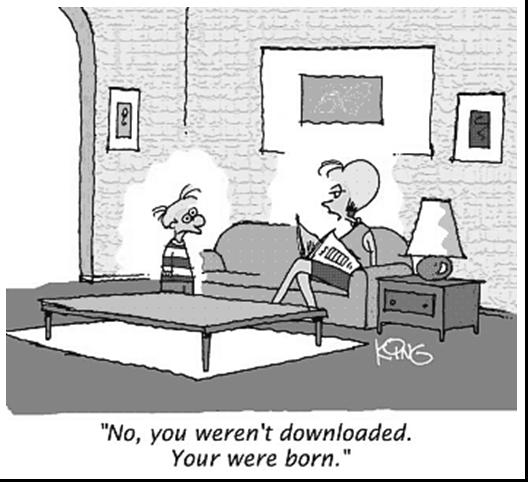
\includegraphics[width=.5\textwidth]{fig1.jpg}
%\caption{A typical figure}
%\label{fig:exampleFig1}
%\end{figure}

%\begin{figure}[ht]
%\centering
%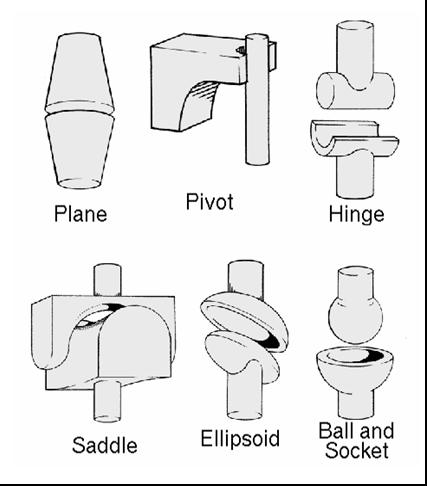
\includegraphics[width=.3\textwidth]{fig2.jpg}
%\caption{This figure is an example of a figure caption taking more than one
%  line and justified considering margins mentioned in Section~\ref{sec:figs}.}
%\label{fig:exampleFig2}
%\end{figure}

%In tables, try to avoid the use of colored or shaded backgrounds, and avoid
%thick, doubled, or unnecessary framing lines. When reporting empirical data,
%do not use more decimal digits than warranted by their precision and
%reproducibility. Table caption must be placed before the table (see Table 1)
%and the font used must also be Helvetica, 10 point, boldface, with 6 points of
%space before and after each caption.

%\begin{table}[ht]
%\centering
%\caption{Variables to be considered on the evaluation of interaction
%  techniques}
%\label{tab:exTable1}
%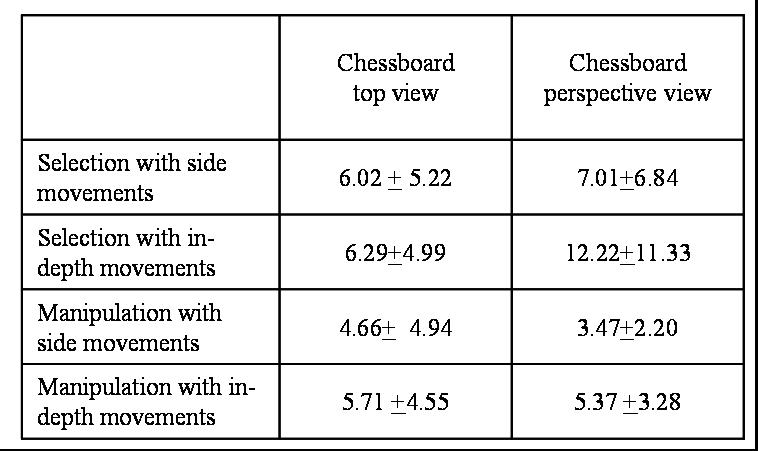
\includegraphics[width=.7\textwidth]{table.jpg}
%\end{table}

%\section{Images}

%All images and illustrations should be in black-and-white, or gray tones,
%excepting for the papers that will be electronically available (on CD-ROMs,
%internet, etc.). The image resolution on paper should be about 600 dpi for
%black-and-white images, and 150-300 dpi for grayscale images.  Do not include
%images with excessive resolution, as they may take hours to print, without any
%visible difference in the result. 

\section{References}

%Bibliographic references must be unambiguous and uniform.  We recommend giving
%the author names references in brackets, e.g. \cite{knuth:84},
%\cite{boulic:91}, and \cite{smith:99}.

%The references must be listed using 12 point font size, with 6 points of space
%before each reference. The first line of each reference should not be
%indented, while the subsequent should be indented by 0.5 cm.

\bibliographystyle{sbc}
\bibliography{sbc-template}

\end{document}
